\section{A motivating example: parkinson's disease}
\label{intro-complete_ex}

need for confrontation
heterogeneous data

spline
heterogeneous data and overlapping age groups \ref{applications-age_groups} \ref{theory-age_group_model-overlapping_data}
study level fixed effects (diagnostic criteria) \ref{applications-efx_study_level} \ref{theory-covariate_modeling}
country level fixed effects (representative) \ref{applications-efx_country_level} \ref{theory-covariate_modeling}
random effects \ref{applications-rfx} \ref{theory-covariate_modeling}
csmr v pf \ref{applicatoins-csmr} \ref



    \begin{figure}[h]
        \begin{center}
            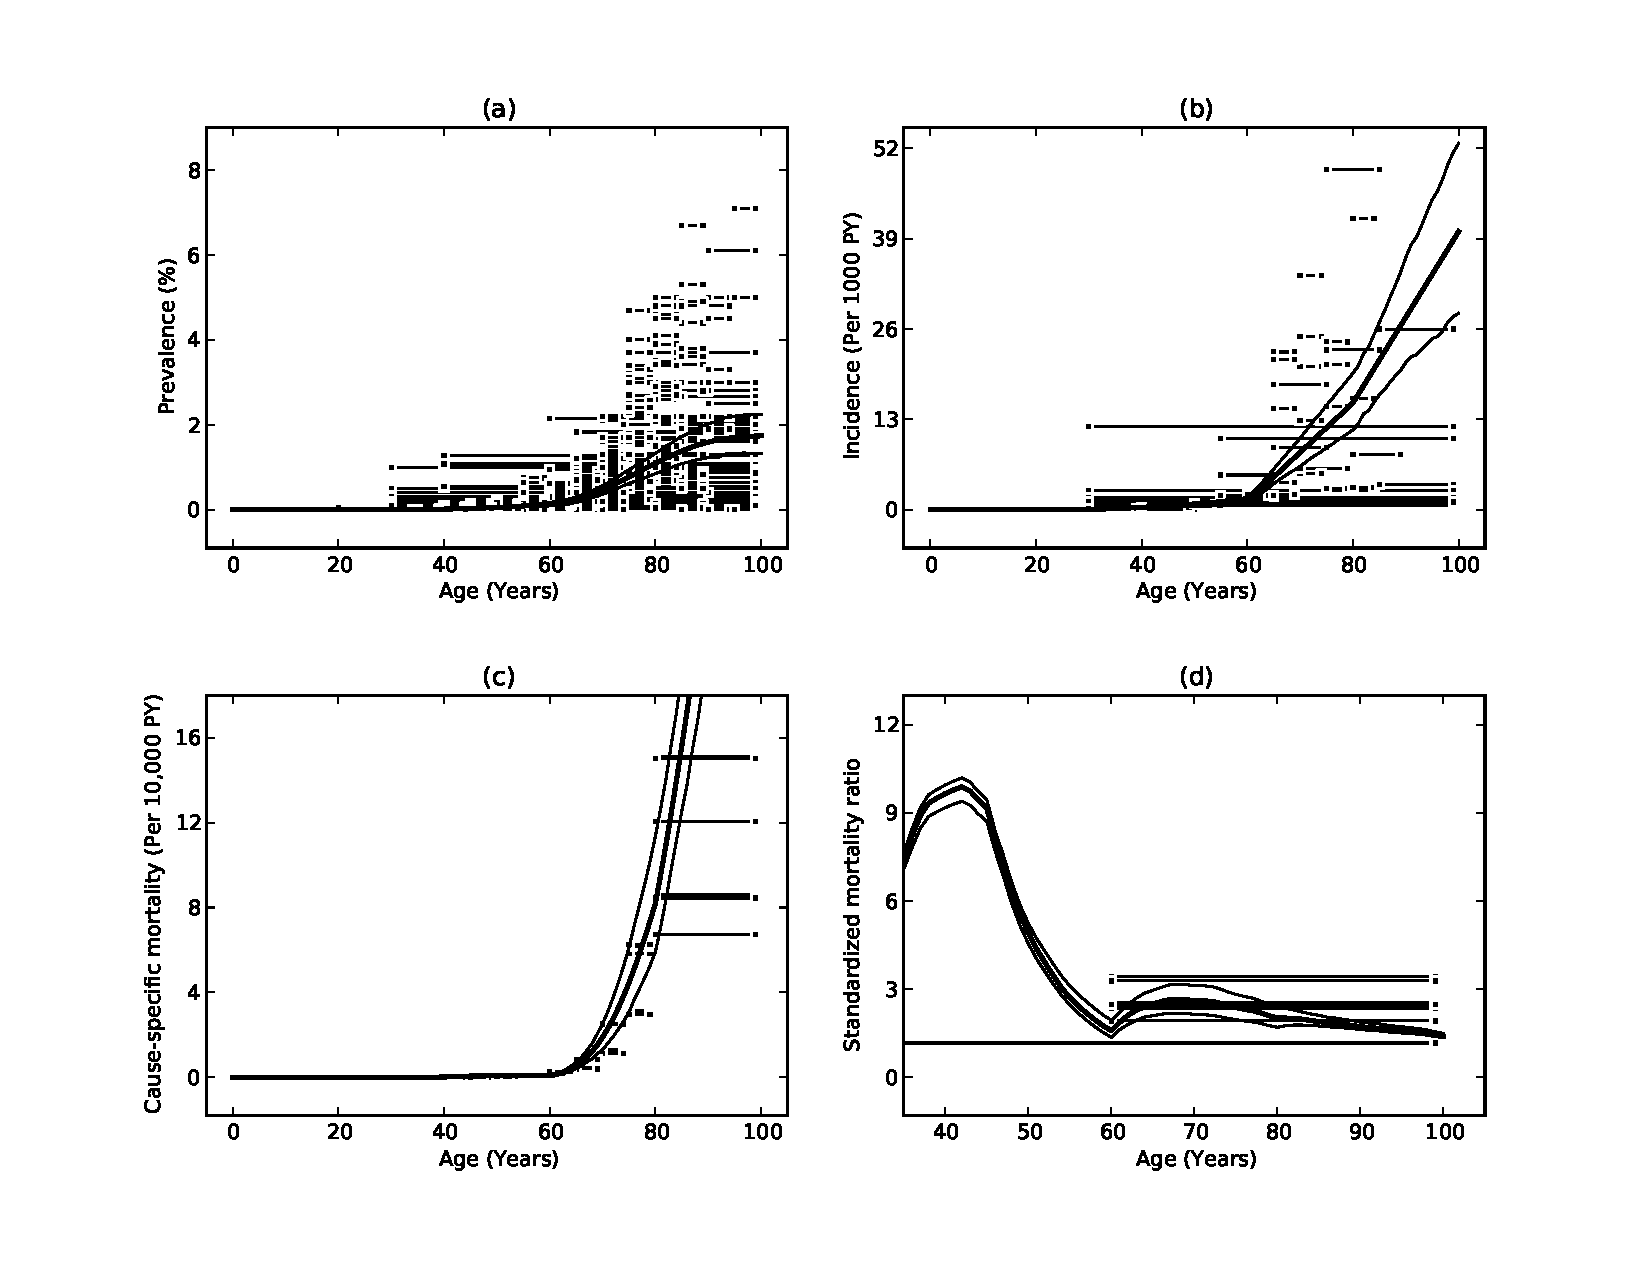
\includegraphics[width=\textwidth]{parkinsons-best.pdf}
            \caption{Estimates of prevalence (panel (a)), incidence (panel (b)), cause-specific mortality (panel (c)) and the standardized mortality ratio of Parkinson's disease in Western European females in 2005.}
            \label{fig:app-fruit rate type}
        \end{center}
    \end{figure} 